\newpage
\section{Durchführung}
\label{sec:Durchführung}

% Was wurde gemessen bzw. welche Größen wurden variiert?

Der Versuchsaufbau ist in \autoref{fig:aufbau} zu sehen und besteht aus einer Röntgenröhre, einem Geiger-Müller Zählrohr und wahlweise einem LiF-Kristall oder einem Plexiglasstreuer.
Zwischen Röntgenröhre und Streuer kann eine Blende eingesetzt werden und an verschiedenen Stellen im Strahlengang kann eine Aluminiumplatte als Absorber eingesetzt werden.

\begin{figure}
    \centering
    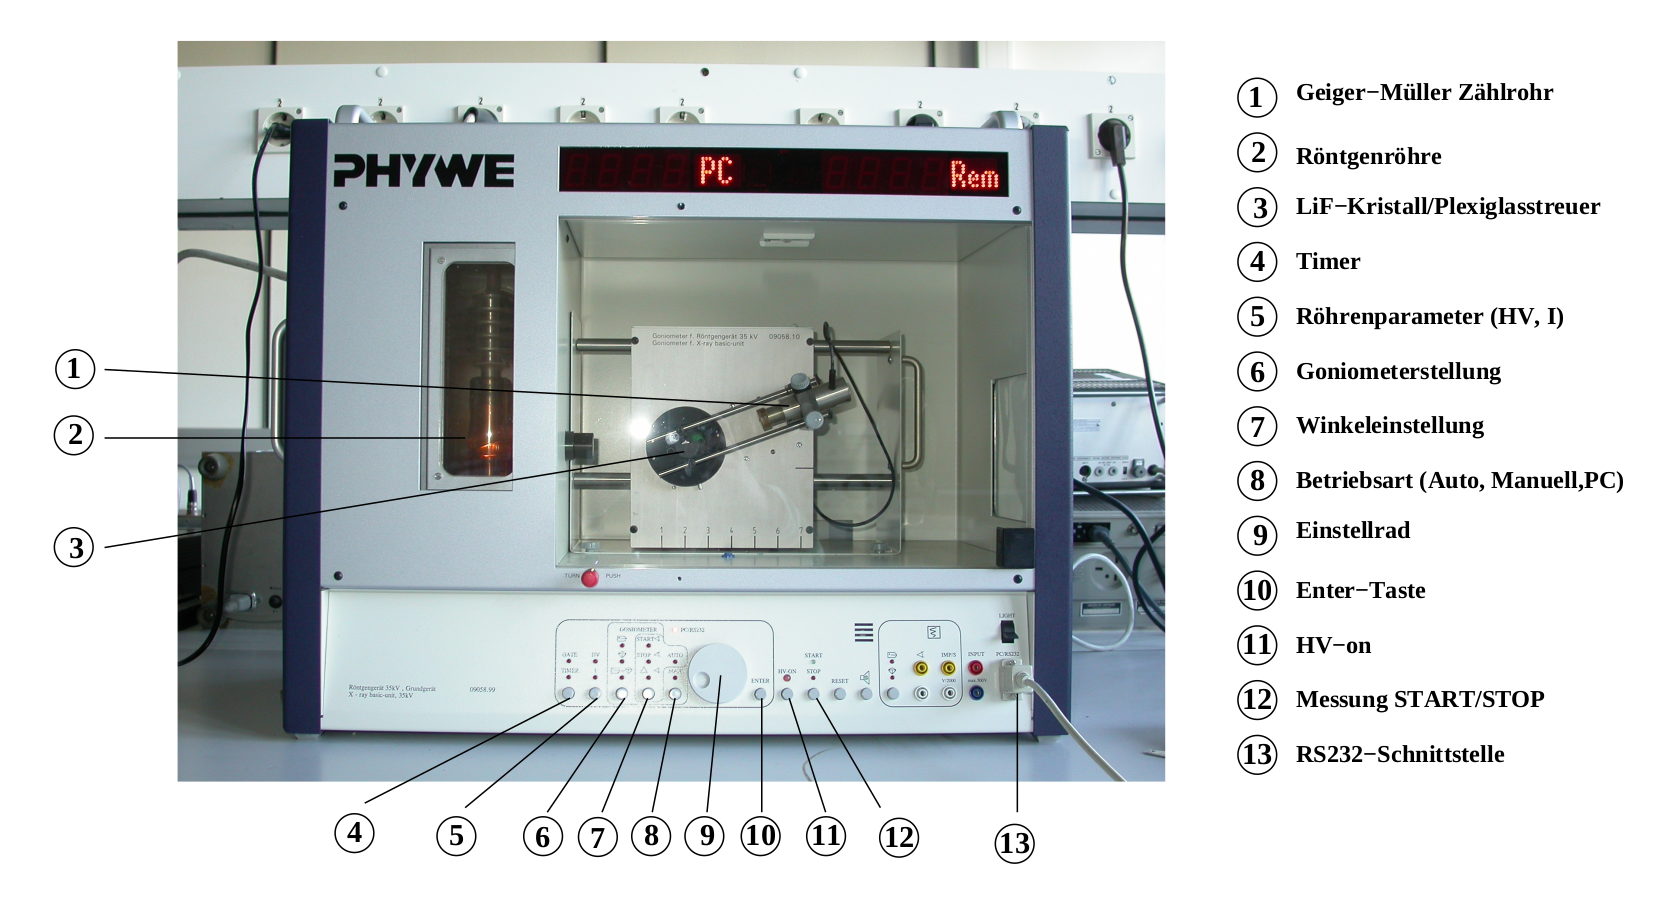
\includegraphics[width=0.5\textwidth]{images/bild_3.png}
    \caption{Versuchsaufbau.\cite{V603}}
    \label{fig:aufbau}
\end{figure}

Um das Emissionsspektrum der Röntgenröhre zu messen, wird der LiF-Kristall und eine $\SI{2}{\milli\metre}$ Blende verwendet.
Es wird in $\Delta \alpha = \SI{0.1}{\degree}$ Schritten von $\alpha=\SI{8}{\degree}$ bis $\alpha = \SI{25}{\degree}$ für je 10 Sekunden gemessen.

\FloatBarrier

Als nächstes wird die Transmission durch eine Aluminiumplatte je Wellenlänge $T(\lambda)$ gemessen.
Dafür wird immernoch mit dem LiF-Kristall die Intensität für $\alpha = \SI{7}{\degree}$ bis $\alpha = \SI{10}{\degree}$ gemessen.
Es wird einmal ohne Aluminiumplatte und einmal mit eingesetzter Aluminiumplatte zwischen Blende und LiF-Kristall gemessen.

\begin{figure}
    \centering
    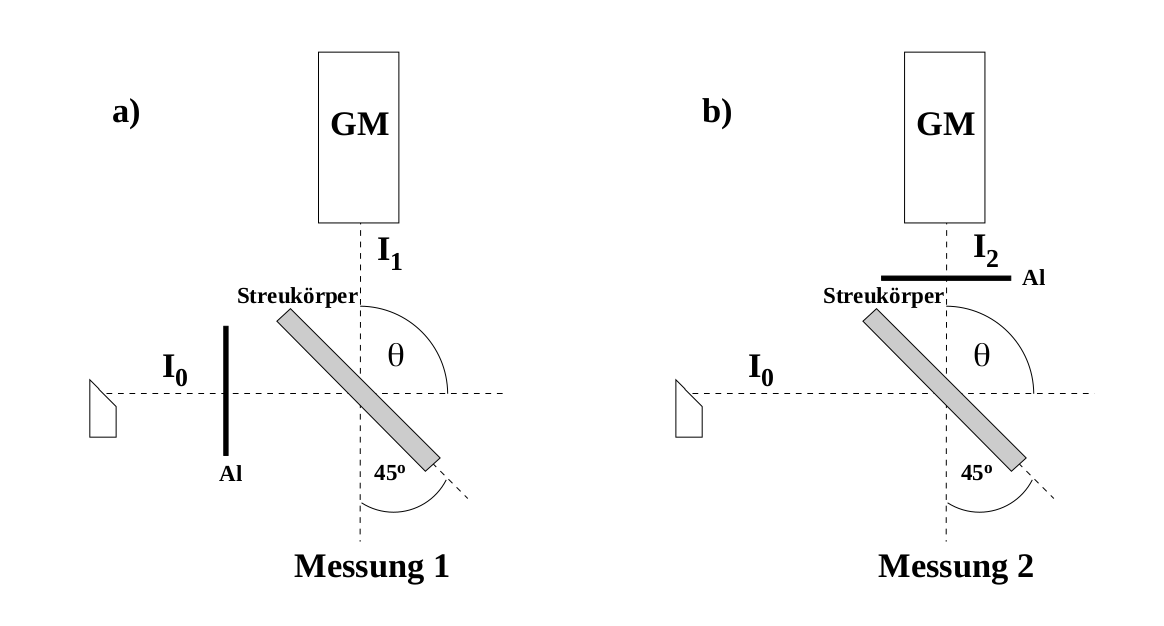
\includegraphics[width=0.5\textwidth]{images/bild_4.png}
    \caption{Schematischer Versuchsaufbau.\cite{V603}}
    \label{fig:schema}
\end{figure}

Um die Compton-Wellenlänge zu bestimmen wird statt LiF-Kristall ein Plexiglasstreuer und statt der $\SI{2}{\milli\metre}$ Blende eine $\SI{5}{\milli\metre}$ Blende verwendet.
Der Kristall wird auf $\SI{45}{\degree}$ und der Geiger-Müller Zähler auf $\SI{90}{\degree}$ gestellt. (siehe \autoref{fig:schema})
Mit diesem Aufbau werden bei einer Integrationszeit von je 300 Sekunden drei Verschiedene Intensitäten gemessen.
Als erstes wird die Intensiät der gestreuten Röntgenstrahlung ohne einen Aluminiumabsorber gemessen.
Dann wird die Intensität gemessen, wenn die Aluminiumplatte zwischen Röntgenröhre und Plexiglasstreuer ist. (\autoref{fig:schema}a)
Und als letztes wird mit der Aluminiumplatte zwischen Plexiglasstreuer und Geiger-Müller Zähler gemessen. (\autoref{fig:schema}b)